\documentclass[letterpaper,twocolumn,10pt]{article}
\usepackage{usenix,epsfig,endnotes}
\usepackage{amssymb}
\usepackage{amsthm}
\usepackage{tabularx}
\usepackage[utf8]{inputenc}
\usepackage{color}
\usepackage{graphicx}
\usepackage{xspace}

\DeclareMathAlphabet{\mathcal}{OMS}{cmsy}{m}{n}

\newcommand{\kyle}[1]{\textcolor{blue}{[[\textsf{Kyle:  #1}]]}}
\newcommand{\fan}[1]{\textcolor{red}{[\textsf{Fan:  #1}]}}
\definecolor{darkgreen}{rgb}{0,0.6,0}
\newcommand{\ari}[1]{\textcolor{darkgreen}{[\textsf{Ari:  #1}]}}
\definecolor{purple}{rgb}{0.75,0,1}
\newcommand{\ethan}[1]{\textcolor{purple}{[\textsf{Ethan: #1}]}}

\newtheorem{lemma}{Lemma}

%don't want date printed
\date{}

%make title bold and 14 pt font (Latex default is non-bold, 16 pt)
\title{\Large \bf Town Crier}

%for single author (just remove % characters)
\author{
{\rm Your N.\ Here}\\
Your Institution
\and
{\rm Second Name}\\
Second Institution
\and
{\rm Name}\\
Name Institution
} % end author


%**** DEFINITIONS *********

\newcommand {\tcs} {Town Crier\xspace}
\newcommand {\tc} {TC\xspace}
\newcommand {\tcontract} {{TContract}\xspace}
\newcommand {\encname} {{Engine}\xspace}
\newcommand {\medname} {{Relay}\xspace}

\newcommand {\reqcont} {${\cal R}$\xspace}
\newcommand {\tcont} {${\cal T}$\xspace}
\newcommand {\tcadd} {${\cal A}$\xspace}
\newcommand {\pkA} {{\sf pk}_{\cal A}\xspace}
\newcommand {\skA} {{{\sf sk}_{\cal A}}\xspace}

\newcommand {\dgreq} {{\sf d.req}\xspace}
\newcommand {\dgform} {{\sf d.form}\xspace}
\newcommand {\dgpay} {{\sf d.pay}\xspace}
\newcommand {\dg} {{\sf d}\xspace}
\newcommand {\dgret} {{\sf d.ret}\xspace}
\newcommand {\dgm} {{\sf d.data}\xspace}
\newcommand {\dgi} {{\sf d.index}\xspace}

%*****************************

\begin{document}

\maketitle

% Use the following at camera-ready time to suppress page numbers.
% Comment it out when you first submit the paper for review.
% \thispagestyle{empty}

\subsection*{Abstract}
Smart contracts are programs that execute autonomously on blockchains. Many of their envisioned uses (e.g., as financial instruments) require them to consume data (e.g., equity prices) from outside the blockchain. Trustworthy data feeds that can interface with smart contracts will thus be a critical component of any smart-contract ecosystem.

	We present an authenticated data feed system called Town Crier (TC). TC builds on the observation that many web sites, such as major news and finance sites, already serve as trusted data sources for non-blockchain uses. TC acts as a bridge between such servers and smart contract systems, using trusted hardware to authenticate and scrape data from HTTPS-enabled websites. While initially designed specifically for the cryptocurrency Ethereum, TC is generalizable to any smart-contract setting and is the first [what can we claim?].
	
	TC delivers authenticated, timestamped datagrams to relying smart contracts. It also includes a range of advanced features, such as private datagrams, which are produced by evaluating encrypted functions supplied by relying contracts within TC's hardware.
	
	%, support for a rich array of trust models on data sources, including options to combine data from multiple sources, and a feature (``deniable datagrams'') for preventing freeloaders from recycling datagrams in a fee-for-service version of TC.
	
	We describe the TC architecture, its underlying trust model, and its applications, and report on an implementation that uses the newly released SGX software development kit. We will soon launch TC as an online public service.
	

\elaine{TODO: change $pk_{TC}$ notation. right now it is inconsistent throughout the paper}

\section{Introduction}

Smart contracts are computer programs that autonomously facilitate or execute a contract. For decades, they have been envisioned as a means to extend the reach of existing contract law and render it more precise and efficiently executable through logical specification of legal agreements. Szabo, who coined the term ``smart contact'' in a seminal 1993 paper~\cite{}, gave as an example a smart contract that enforces car loan payments. If the owner of the car fails to make a timely payment, a smart contract could revoke physical access and return control of the ignition key to the bank. The contract could additionally be programmed to do so only at a time that is safe for the the owner, e.g., while the car is parked.

The emergence of decentralized cryptocurrencies such as Bitcoin has created new opportunities to realize smart contracts, thanks to two properties. First, cryptocurrencies equate control of their assets with knowledge of a private cryptographic key, in principle making control of money possible by an arbitrary computer program such as a smart contract. Second, cryptocurrencies are built atop blockchains, whose state evolves through a consensus protocol that treats transactions as computations over a global data structure. As these computations are decentralized, a blockchain may be viewed as an idealized abstraction equivalent to a trusted third party. It ensures fair, automated execution of computations over global state and eliminates the need for trusted intermediaries. 

While the scripting language embodied in Bitcoin is intentionally limited (e.g., lacks support for loops), the recently launched decentralized cryptocurrency Ethereum supports Turing-complete code. Ethereum can thus in principle realize fully expressive, self-enforcing, and self-executing smart contracts, going a long way toward fulfilling the vision of researchers and proponents.  

As Szabo's example shows, though, the most compelling applications of smart contracts cannot be realized in isolation on a blockchain, but require access to data about real-world state and phenomena. Financial contracts and derivatives, perhaps the most commonly cited applications of Ethereum~\cite{}, must be able to consume data about financial markets, including equity and commodity prices and exchange rates. Applications such as insurance policies are only realizable with data about weather, flights, delivery of goods, and so forth. 

To meet this need, the architects of Ethereum have proposed the use of \emph{data feeds} (sometimes called ``oracles''), contracts on the blockchain that serve data requests by other contracts~\cite{whitepaper,yellowpaper}. A few such data feeds, such as PriceFeed and Oraclize.it, support Ethereum smart contracts today, but have a notable drawback: They provide no assurance of trustworthy data beyond the reputation of their operators (who are typically individuals or small entities), even if their is data ultimately obtained from trustworthy sources.\footnote{Oraclize.it itself makes use of TLSnotary to notarize data, thereby distributing trust across two (small) operators.\ari{I think TLSnotary just signs webpages. So it's not clear how the mapping from pages to data is authenticated.}} To address this problem, systems such as SchellingCoin and Augur~\cite{} have been proposed that rely on mechanisms such as prediction markets to decentralize trust. While decentralization of trust is attractive, and underpins cryptocurrencies to begin with, prediction markets can support only a limited number of data feeds and have not yet seen widespread use in cryptocurrencies. The lack of a substantive ecosystem of trustworthy data feeds in Ethereum indeed remains a critical obstacle to its evolution~\cite{???}.

At the same time, however, existing e-commerce already relies on a wealth of broadly trusted data available from existing sources, namely websites operated by generally reputable organizations. The sources of such data, moreover, can be authenticated by a client if served over HTTPS. Smart contracts, however, cannot directly access internet data, as they do not have network access.

We present a system called \emph{Town Crier} (\tc) that fills the gap between smart contracts and today's data sources by serving as what we call an \emph{authenticated data feed} (ADF). \tc functions as a bridge between existing HTTPS-enabled data sources and the Ethereum blockchain, retrieving data from these sources and serving it to relying contracts on the blockchain in the form of specific data items that we call \emph{datagrams}. \tc avoids the problem of bootstrapping trust by executing its core functionality in an environment protected by \emph{trusted hardware}. Specifically, \tc makes use of Intel's recently released Software Guard Instructions (SGX). SGX enables a server to run a piece of code $\prog$ in an isolated environment called an \emph{enclave} (protected against even a malicious OS) and \emph{attest} (prove) to a remote party that the party is interacting with a legitimate, SGX-backed instance of $\prog$. 

By operating through a smart-contract front end, \tc can thus furnish a requested datagram $X$ from a particular trusted source, e.g., \texttt{https://www.Y.com}, such that a relying contract $\cont$ can authenticate that $X$ came from $Y$ assuming only that: (1) $\prog$ correctly retrieves and serves data and (2) The \tc server's hardware has not been tampered with. (Of course, there is also a need to trust Intel, which serves as a root of trust for SGX-enabled hosts in general.) Note that trust in $Y$ itself is orthogonal, and \tc can combine data sources according to any desired policy (e.g., majority voting across sources).

While conceptually simple, \tc presents a number of technical challenges. First, there are implementation challenges in securely interfacing enclave code with the blockchain and with data sources. Ethereum lacks native support for and therefore does not permit efficient on-chain verification of the proprietary digital signatures SGX uses to generate attestations on enclave code. Enclave code cannot directly scrape blockchain data and must instead rely on an untrusted process to retrieve correct blockchain data.\footnote{This problem cannot be solved by the obvious mechanism of digitally signing blockchain data: The blockchain is globally readable, and thus cannot store private keys, and running a blockchain client in the enclave would bloat the TCB in the enclave unacceptably.} Additionally, for enclave code to communicate securely with data sources, it must do so over HTTPS, yet enclave code in SGX does not control the host's network stack, which is instead controlled by the (potentially untrusted) OS. A second challenge is in the proofs of security for \tc. These proofs require harmonized formalism for SGX and smart contracts that existing work does not yet provide. Moreover, Ethereum requires expenditure of a currency-derived resource known as \emph{gas} to power contracts; thus proving the availability of \tc---a critical property for relying contracts---requires conventional analysis of data integrity coupled with a proof of sustainable gas expenditure. Finally, the use of \tc raises confidentiality challenges. Since blockchain state is globally readable, na\"{i}ve use of \tc would expose potentially sensitive datagram requests, e.g., an flight-insurance policy would publicly reveal the flight information of policyholders, and would render \tc vulnerable to traffic analysis on served data. Much of our contribution in the design of \tc involves addressing these challenges. 

Beyond merely serving publicly visible requests for generic data, \tc supports private datagram requests in which the request is encrypted and custom datagram requests in which the requested data comes from an access-controlled system, such as an individual user's account. Thus \tc can support a rich variety of smart contracts, as shown by our implementation of three example contracts: (1) A financial derivative (cash-settled put option) that requires stock ticker data; (2) A flight insurance contract that relies on private data requests about flight cancellations; and (3) A contract for exchanging currency in an online role playing game for ether, the Ethereum currency, using custom data requests.

In summary, our contributions are as follows:

\vspace{-1mm}
\begin{itemize}
  \setlength{\itemsep}{2pt}
  \setlength{\parskip}{0pt}
  \setlength{\parsep}{0pt}

\item \emph{\tcs system:} We present and describe our implementation of \tc, an authenticated data feed system that enables smart contracts to obtain datagrams safely from a target data source, specifically an existing HTTPS-enabled server. In contrast to currently available systems, \tc's assurances do not require trust in (typically fledgling) service operators, only in the underlying commodity trusted hardware, namely Intel SGX. 

\item \emph{Interfacing SGX with smart contracts:} We present solutions to the technical challenges that arise in combining two new technologies with incompatible APIs, e.g., the lack of Ethereum support for SGX attestations and the impracticality of authenticating blockchain data, and thus datagram requests, to \tc's trusted enclave program. 

\item \emph{\tc security analysis:} We present unifying formalism for the trusted hardware and smart contracts embodied in \tc and provide proofs of security, including the integrity and source authenticity of datagrams and service availability, which requires a new form of analysis of sustainable gas consumption. 

\item \emph{\tc applications:} We implement three practical smart contract applications that benefit from \tc: a financial derivative, a flight insurance contract, and a contract for exchanging online game currency and cryptocurrency. These applications showcase the rich possibilities and capabilities of \tc, including support for private and custom datagrams. 

\end{itemize}

As \tc has minimal trust assumptions and requires no modification to existing data source servers or Ethereum, we believe it offers a compelling, practical approach to bootstrapping a data feed ecosystem for smart contracts.



%\vspace{-3mm}
\section{Background}
\label{sec:background}

In this section, we provide basic background respectively on the main technologies \tc incorporates, namely SGX, TLS / HTTPS, and smart contracts.

%\vspace{-2mm}
\paragraph{\bf SGX.}
Intel's Software Guard Extensions (SGX)~\cite{sgx,sgxfordummy,mckeen2013sgx,anati2013sgx,hoekstra2013sgx} is a set of new instructions that confer hardware protections on user-level code. SGX enables a process to execute in a protected address space known as an {\em enclave}, which protects the confidentiality and integrity of the process from other software on the same host, including the operating system, and certain forms of hardware attack. 

A enclave process cannot make system calls, but can read and write memory outside the enclave region. Thus isolated execution in SGX may be viewed in terms of an ideal model in which a process is guaranteed to execute correctly and with perfect confidentiality, but relies on a (potentially malicious) operating system for network and file-system access.\footnote{This model is a simplification: SGX is known to expose some internal enclave state to the OS~\cite{sgxexplained}. Our basic security model for \tc assumes ideal isolated execution, but again, \tc can also be distributed across multiple SGX instances as a hedge against compromise.}

SGX allows a remote system to verify the software in an enclave and communicate securely with it. When an enclave is created, the CPU produces a hash of its initial state known as a {\em measurement}. The software in the enclave may at a later time request a report, which includes a measurement and supplementary data provided by the process, such as a public key. The report may be digitally signed using a hardware-protected key to produce a proof that the measured software is running in an SGX-protected enclave. This proof, known as a {\em quote}, may be verified by a remote system, while the process-provided public key can be used by the remote system to establish a secure channel with the enclave or verify signed data it emits. We use the generic term {\em attestation} to refer to a quote, and denote it by \att. We assume that a trustworthy measurement of the code for the enclave component of \tc is available to any client that wishes to verify an attestation. SGX signs quotes using a \emph{group signature} scheme called 
EPID~\cite{epid}. This choice of primitive is significant in our design of \tcs, as EPID is a proprietary signature scheme not supported in Ethereum.

SGX additionally provides a trusted time source via the function \texttt{sgx\_get\_trusted\_time}.~On invoking this function, an enclave obtains a measure of time relative to a reference point indexed by a nonce. A reference point remains stable, but SGX does not provide a source of absolute or wall-clock time, a limitation that we must work around in \tc.

%\vspace{-2mm}
\paragraph{\bf TLS / HTTPS.}
We assume basic familiarity by readers with TLS and HTTPS (HTTP over TLS). As we explain later, \tc exploits an important feature of HTTPS, namely that it can be partitioned into interoperable layers: An HTTP layer interacting with web servers, a TLS layer handling handshakes and secure communication, and a TCP layer providing reliable data stream. 

%\vspace{-2mm}
\paragraph{\bf Smart contracts.}
\label{sec:contracts-and-gas}
While \tc can in principle support any smart-contract system, we focus in this paper on its use in Ethereum, whose use we now explain. For further details, see~\cite{whitepaper,yellowpaper}

A smart contract in Ethereum is represented as what is called a \emph{contract account}, endowed with code, a currency balance, and persistent memory in the form of a key/value store. A contract accepts messages as inputs to any of a number of designated functions. These entry points, determined by the contract creator, represent the API of the contract. Once created, a contract executes autonomously; it persists indefinitely, with even its creator unable to modify its code.\footnote{There is one exception: A special opcode \texttt{suicide} wipes code from a contract account.} Contract code executes in response to receipt of a \emph{message} from another contract or a \emph{transaction} from a non-contract (\emph{externally owned}) account, informally what we call a \emph{wallet}. Thus, contract execution is always initiated by a transaction. Informally, a contract only executes when ``poked,'' and poking progresses through a sequence of entry points until no further message passing occurs (or a shortfall in gas occurs, as explained below). The ``poking'' model aside, as a simple abstraction, a smart contract may be viewed as an {\em autonomous agent} on the blockchain.

Ethereum has its own associated cryptocurrency called \emph{ether}. (At the time of writing, 1 ether has a market value of a little more than \$5 U.S. \cite{ethprice}.)  To prevent Denial-of-Service (DoS) attacks, inadvertent infinite looping within contracts, and generally to control network resource expenditure,
Ethereum allows ether-based purchase of a resource called \emph{gas} to power contracts.
Every operation, including sending data, executing computation, and storing data, has a fixed gas cost.
Transactions and messages include a parameter (\texttt{GASLIMIT}) specifying a bound on the amount of gas expended by the computations they initiate.
When a function call is made, the child function expends gas from the same source as the parent function.
Should a function fail to complete due to a gas shortfall,
it is aborted and any state changes induced by the partial computation are rolled back to their pre-call state;
previous computations on the call path, though, are retained.

Along with a \texttt{GASLIMIT}, a transaction specifies a \texttt{GASPRICE}, the maximum amount in ether that the transaction is willing to pay per unit of gas. The transaction thus succeeds only if the initiating account has a balance of \texttt{GASLIMIT} $\times$ \texttt{GASPRICE} ether and \texttt{GASPRICE} is high enough to be accepted by the system (miner). 

The management of gas, as we show in our design of \tcs can be delicate. Without careful construction, \tc's smart contract front end on the Ethereum blockchain can be caused by an attacker to exhaust the ether used to power the delivery of datagrams.

Finally, we note that transactions in Ethereum are digitally signed for a wallet using ECDSA on the curve Secp256k1 and the hash function SHA3-256.




 \section{\tc Architecture and Security Model}

%In this section, we discuss the general design of \tc. First we present a strawman system design that illustrates some of the technical challenges that arise in the design of \tc. We then present our \tc architecture, describing the front-end (blockchain) and back-end (off-chain) components, and give a high-level view of the security model underpinning our design.

\iffalse{
\subsection{Strawman design}

Here we sketch a simple (but, as we show, na\"{i}ve) strawman design that provides authenticated data feeds along with accompanying attestations. 

%To harmonize with terminology introduced shortly in the paper, we refer to the untrusted component of a \tc host as the \medname and the code running in an SGX enclave as the \encname.

The strawman solution is as follows:

\begin{itemize}[leftmargin=5mm]
\item
{\bf Monitor and relay.}
The \tc system
monitors the blockchain for 
datagram requests. A contract \reqcont 
requests a datagram by including a distinguished message in its state (e.g., ``\tc service \#123 request:''), along with
a specification \dgform of the requested datagram.
Monitoring happens in the untrusted part of the \tc server, which controls the network stack. Any scraped specification \dgform is passed to a (trusted) enclave process.
\item
{\bf Securely fetch feed.}
Based on the \dgform, the trusted enclave process contacts a data source, establishing an HTTPS channel to a suitable target web page $\weburl$ (which might, e.g., be specified in \dgform). 
The process verifies that the validity of the certificate for the host serving \weburl.
It then fetches page contents, parses them, and extracts a datagram \dgm as specified in \dgform.

Finally, the enclave process produces an attestation $\att$ on: its code in the enclave, $\dgform$, a timestamp $T$ on the fetched data, and $\dgm$. 
It sends $\att$ to $\reqcont$.
\item
{\bf Verify}.
\reqcont verifies the attestation $\att$. If successful, \reqcont consumes \dgm (potentially matching \dgform against an internal queue of datagram requests).
\end{itemize}

This strawman scheme has a few nice features: conceptual simplicity, no need to maintain a \tc contract on the blockchain, and the ability for \reqcont to check the freshness of \att. It has a few serious drawbacks, however.

\paragraph{Problems with the strawman scheme.}
Our strawman scheme is unworkable for several reasons. First, verification of \att in the requesting contract \reqcont is not practical. Although SGX provides a 
trusted clock, the clock does not provide absolute time, but only time relative to a host-specific reference point.
Thus it is not clear in our strawman scheme how to produce a timestamp $T$ in absolute time. Furthermore, in Ethereum, opcodes for in-contract cryptographic operations are very limited and do not support the proprietary EPID group-signature scheme present in SGX attestations. While achievable in principle, as the Ethereum virtual machine is Turing-complete, verification of attestations would impose prohibitively expensive gas costs on \reqcont. 

To address these problems, our \tc architecture supports only off-chain verification of attestations.

Another problem with our strawman scheme is that it lacks an on-blockchain mechanism to enforce payment for datagrams. It is desirable for \tc to accept payments via a smart contract in order to permit payment in the system's cryptocurrency (e.g., Ether) and to ensure a {\em fair exchange} between payments and datagrams. Even a not-for-profit \tc service might accept small gas payments to cover the cost of datagram transmission. Without enforcement of fair exchange, relying contracts or the \tc service would risk being defrauded by the other party. \tc could attempt to deliver datagrams only to contracts whose code guarantees payment to \tc, but verifying this property even in templated code would be challenging, given the many complicated dependencies in a smart-contract system (e.g., a contract might attempt to make payment but lack gas or ether). 

To address these problems, our \tc architecture uses a smart contract \tcont as a blockchain front end.
\fi

The \tcs system includes three main components: The \tcontract (\tcont), the \encname (\engine), and the \medname (\relay). The \encname and \medname reside on the \tc server, while the \tcontract  resides on the blockchain. An architectural schematic showing the roles of these components is given in Figure~\ref{fig:overview}.

\vspace{-2mm}
\begin{figure}[h!]
\centering
\begin{tikzpicture}
  [entity/.style={rectangle,draw=black,minimum height=3.5em,text width=3.5em,align=center},
   contract/.style={entity,text width=5.7em},
   trusted/.style={fill=green!30},
   communication/.style={blue,ultra thick,text=black},
   bg-box/.style={rectangle,rounded corners,draw=black,dashed}]
  \node[contract,trusted] (ctc) {TC Contract\\$\tcont$};
  \node[contract,fill=white,below=1.5em of ctc] (cu) {User Contract\\$\reqcont$};
  \node[entity,fill=none,right=2.5em of ctc] (relay) {Relay};
  \node[entity,trusted,right=2.5em of cu] (enc) {Enclave};

  \begin{pgfonlayer}{background}
    \node[bg-box,
          fill=yellow!20,
          fit={($(ctc.north east)+(0.25em,0.25em)$)($(cu.south west)+(-0.25em,-0.25em)$)},
          label=above:{\bf Blockchain}] (blockchain) {};
    \node[bg-box,
          fill=black!20,
          fit={($(relay.north east)+(0.25em,0.25em)$)($(enc.south west)+(-0.25em,-0.25em)$)},
          label=above:{\bf TC Server}] (tc) {};
  \end{pgfonlayer}

  \node[right=-0.15em of tc,color=red,transform canvas={yshift=2.5em}] (https) {\scriptsize \bf HTTPS};
  \node[rectangle,draw=black,fill=red!20,right=2.75em of tc,minimum height=9.75em,label=above:{\bf Data Source}] (data) {\scriptsize \tt LotsOData.com};

  \draw[stealth-stealth,communication] ([xshift=-0.75em,yshift=-0.75em]ctc.east) -| ([xshift=-0.75em,yshift=-0.75em]enc.north);
  \draw[stealth-stealth,communication] ([yshift=0.75em]ctc.south) -- ([yshift=-0.75em]cu.north);
  \draw[stealth-stealth,communication] ([xshift=0.75em,yshift=-0.75em]enc.north) |- ([xshift=0.75em,yshift=1.75em]data.west);
\end{tikzpicture}
\caption{{\bf Basic Town Crier architecture.}}
\label{fig:overview}
\end{figure}

%\begin{figure}[h!]
%\centering
%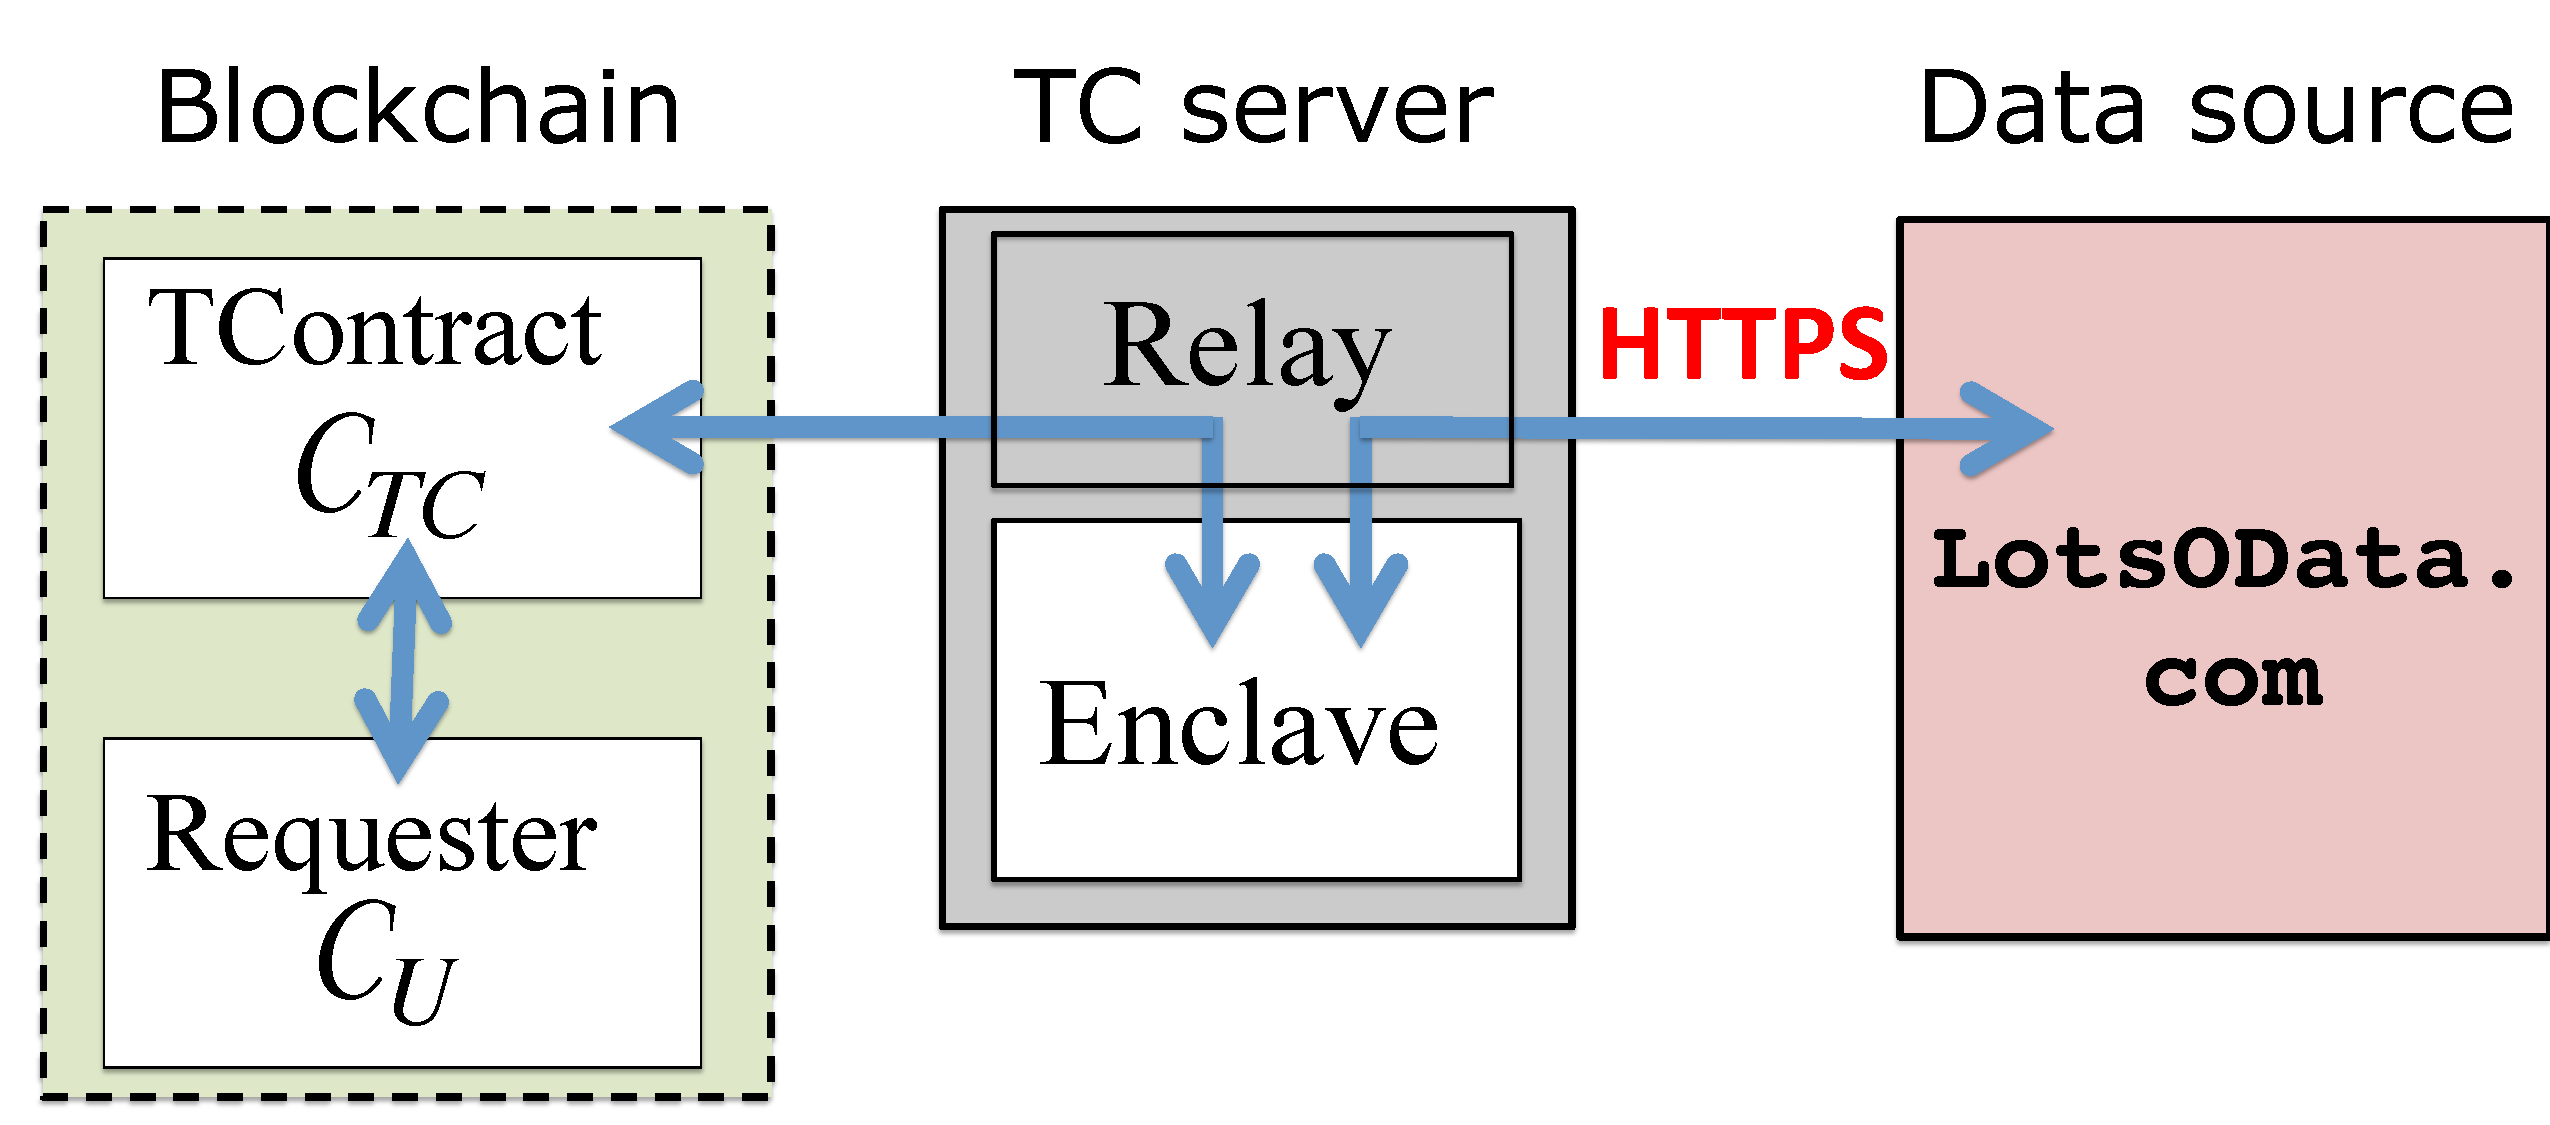
\includegraphics[width=\columnwidth]{figures/OverviewFig}
%\caption{{\bf Basic Town Crier architecture.}}
%\label{fig:overview}
%\end{figure}
\vspace{-2mm}

\paragraph{The \tcontract \tcont.} The \tcontract (denoted by \tcont) is a smart contract that acts as the blockchain front end of the \tc service. It is designed to present a simple API to a relying contract \reqcont for its requests from \tc. Very simply, \tcont accepts datagram requests from a requester \reqcont and returns corresponding datagrams from \tc. Additionally, \tcont manages \tc monetary resources, which in Ethereum take the form of ether (money) and gas (``fuel'' for contracts).

\paragraph{The \encname \engine.}
We refer to the TC code running in the SGX enclave simply as the \encname. In TC, the \encname ingests and fulfills datagram requests from the blockchain. To obtain the data for inclusion in datagrams, it queries external data sources, specifically HTTPS-enabled internet services. It returns a datagram to a requesting contract \reqcont as a digitally signed blockchain message. Under our assumed security model for SGX, apart from its network functions, the \encname runs in complete isolation from an adversarial OS as well as other process on the host. 

\paragraph{The \medname \relay.} As an SGX enclave process, the \encname lacks direct network access. Thus the \medname handles bidirectional network traffic on behalf of the \encname. Specifically, the \medname provides network connectivity from the \encname to three different types of entities: 

\begin{enumerate}
\item {\em The Blockchain (the Ethereum system):}  The \medname scrapes the blockchain in order to monitor the state of the \tcontract  \tcont. In this way, it performs implicit message passing from \tcont to the \encname, as neither component itself has network connectivity. Additionally, the \medname places messages emitted from the \encname (datagrams) on the blockchain.
\item {\em Clients:} The \medname runs a web server to handle off-chain service requests from clients, specifically, requests for attestations from the \encname. As we soon explain, an attestation provides a unique public key for the \encname instance to the  client and proves that the \encname is executing correct code in an enclave and that its clock is correct in terms of absolute (wall-clock time). A client that successfully verifies an attestation can then safely create a relying contract \reqcont that uses the \tc.
\item {\em Data sources:} The \medname relays traffic to and from data sources (HTTPS-enabled servers) queried by the \encname. 
\end{enumerate}

The \medname is an ordinary user-space application. It does not benefit from integrity protection by SGX and thus, unlike the \encname, can be subverted by an adversarial OS on the \tc server, causing network delays or failures. A key design aim of \tc, however, is that \medname should be unable to cause incorrect datagrams to be produced or users to lose fees paid to \tc for datagrams (although they may lose gas used to fuel their requests). As we shall show, in general the \medname~{\em can only mount denial-of-service attacks against \tc}. 

\paragraph{Security model}

Here we give a brief overview of our security model for \tc, providing more details in later sections. We assume the following:

\begin{itemize}

\item {\em Blockchain communication.} Transaction and message sources are authenticable, i.e., a transaction $m$ sent from an account ${\cal P}_{X}$ (or message $m$ from contract ${\cal C}_{X}$) is identified by the receiving account as originating from $X$. Transactions and messages are integrity protected (as they are digitally signed by the sender), but not confidential. 

\item {\em \encname security:} We make three assumptions about \encname : (1) The \encname behaves honestly, i.e., correctly executes the \tc protocol; (2) The private key $\skTC$ is known only to the \encname; and (3) The \encname has an accurate (internal) real-time clock. (Specifically, the clock is accurate to within \ari{XXX}, as we show experimentally.)  We explain in the next section how we achieve these properties through use of SGX and how the public key $\pkTC$ may be bound to an Ethereum account, given the \encname an authenticable blockchain presence. 

\item {\em Network communication.} The \medname (and other untrusted components of the \tc server) can tamper with or delay communications to and from the \encname. (As we explain in our SGX security model, the \medname cannot otherwise observe or alter the behavior of the \encname.) Thus the \medname is subsumed by an adversary that controls the network. 

\end{itemize}













\section{Applications: Requesting Contracts}

\paragraph{Financial derivative ({\sf CashSettledPut}).} Financial derivatives are one of the most commonly cited applications of Ethereum, and exemplify the need for a data feed on financial instruments (specifically, stocks). We implemented an example contract {\sf CashSettledPut} for what is called a {\em cash-settled put option}. This an offer to sell an asset (stock) at an agreed price on or before a particular expiration date (in anticipation of a price drop). It is ``cash-settled'' in that the sale is implicit, i.e., no stock changes hands, only cash reflecting the stock's value. In our implementation, the issuer of the option specifies a strike price $P_S$, expiration date, unit price $P_U$, and maximum number of units $M$ she is willing to sell. A customer may send a request to the contract specifying the number $X$ of option units to be purchased and containing the associated fee ($X \times P_U$). A customer may then exercise the option by sending another request prior to the expiration date. {\sf CashSettledPut} calls \tc to retrieve the closing price $P_C$ of the underlying instrument on the day the option was exercised, and pays the customer $X \times (P_S - P_C)$. To ensure sufficient funding to pay out, the contract must be endowed with ether value at least $M \times P_S$.

\iffalse
\paragraph{Financial Derivatives.}  In order to implement a financial derivative as a smart contract, we require information about the corresponding financial instrument upon which the derivative depends (typically a stock).  As an example, we implemented a cash-settled put option.  The issuer of the option creates a contract for a particular stock, strike price, time period, unit price, and the maximum number of units he is willing to sell.  Customers may purchase the option by sending requests to the contract along with the associated fee indicating the number of units of the option they would like to buy.  Until the expiration date, customers may choose to exercise the put option by making another request to the option contract.  The contract then requests that TC retrieve the closing price of the underlying instrument on the day the option was exercised, and pays out to the customer the difference between the strike price and the closing price for each unit of the option purchased.  To ensure the contract always has sufficient funds to pay out, it must control value of at least the strike price times the maximum number of units sold.
\fi

\paragraph{Flight insurance ({\sf FlightIns}).} Flight insurance indemnifies a purchaser should her flight be delayed or canceled. We have implemented a simple flight insurance contract called {\sf FlightIns}. Our implementation showcases \tc's private-datagram feature to address an obvious concern:  That customers may not wish to reveal their travel plans publicly on the blockchain. 

An insurer stands up {\sf FlightIns} with a specified policy fee, payout, and lead time $\Delta T$. ($\Delta T$ is set large enough to ensure that a customer can't anticipate flight cancellation or delay due to weather, etc.) To purchase a policy, a customer sends the {\sf FlightIns} a ciphertext  $C$ under the \tc's pubic key $\pkTC$ of the ICAO flight number $FN$ and scheduled time of departure $T_D$ for her flight, along with the policy fee. {\sf FlightIns} sends \tc a private-datagram request containing the current time $T$ and the ciphertext $C$. \tc decrypts $C$ and checks that the lead time meets the policy requirement, i.e., that $T_D - T \geq \Delta T$. \tc then scrapes a flight information data source at time $T_D$ to check the flight status, and returns to {\sf FlightIns} predicates on whether the lead time was valid and whether the flight has been delayed or cancelled. If both predicates are true, then {\sf FlightIns} returns the payout to the customer. Note that $FN$ is never exposed in the clear.

Despite the use of private datagrams, {\sf FlightIns} as described here still poses a privacy risk, as the {\em timing} of the predicate delivery by \tc leaks information about $T_D$, which may be sensitive information; this, and the fact that the payout is publicly visible, could also indirectly reveal $FN$. {\sf FlightIns} addresses this issue by including in the private datagram request another parameter $t > T_D$ specifying the time at which predicates should be returned. By randomizing $t$ and making $t - T_D$ sufficiently large, {\sf FlightIns} can substantially reduce the leakage of timing information. 

\iffalse
\paragraph{Flight insurance.} Flight insurance, which provides a payout to the purchaser in the event that their flight is delayed or canceled, is a particularly interesting application of smart contracts as it requires  the transmission of data that the customer may wish to keep private, such as the flight number, via the blockchain.  In order to maintain data privacy, TC supports encrypted datagram requests in which customers encrypt sensitive query information under a public key held by the \encname prior to publicly posting it to the blockchain.  \encname code is then responsible for decrypting and carrying out the query and passing a result back to the requesting contract stripped of private information.  

In the case of the flight insurance contract we implemented, an insurance provider creates an insurance contract with a specified fee and payout in ether that serves up to $2^{64}$ requests.  A customer who wishes to buy insurance for his flight first encrypts the ICAO flight number and scheduled time of departure for his flight, and attaches the ciphertext to a transaction he submits to the insurance contract.  If the transaction has value in ether equivalent to the fee, the contract logs the request and submits the provided ciphertext as a request to TC.  \encname code then decrypts and processes the request, determines if the specified flight was delayed or canceled, and returns a response to the insurance contract indicating whether or not the contract should pay out for a particular request.  Note that there is no flight information contained in this response.

However, the publicly visible outcome of the contract may leak information about which flight a particular customer was on, especially if the customer received a payout for flight cancellation.  An adversary attempting to compromise privacy may then narrow his search to a list of recently canceled flights.  This can be partially solved by including two encrypted addresses in the request, one owned by the customer and one owned by the insurance provider.  The \encname passes back to the requesting contract the customer-owned address if the flight is canceled, and the provider-owned address otherwise.  The contract then makes the payout to the returned address, and the adversary gains no new information from the payment so long as he cannot distinguish between the two addresses.
\fi

\paragraph{Steam Marketplace.} Steam \kyle{reference?} is an online gaming platform that supports thousands of games and maintains its own marketplace, where users can trade, buy, and sell games and other virtual items.  Through the Steam trading API, for which a key is issued to each user, we can construct a contract that implements the sale of games and items for ether using custom datagrams.  A user wishing to sell items creates a contract specifying the items to be sold along with a price in ether for each.  A user wishing to buy the items creates a Steam trade offer requesting the items (which the seller must accept out of band through either a Steam client or the Steam API), and then submits an Ethereum transaction with value in ether equal to the specified price along with an attached ciphertext containing a reference to the trade offer and his Steam API key.  The API key of either the buyer or the seller is required in order to view the contents of the trade.  The contract submits a request to TC using the provided ciphertext, and relies on TC to verify the contents and status of the trade and return the result.  If the trade was successfully accepted by the seller and the items transferred to the buyer, then the contract transfers the buyer's ether to the seller's account.  Otherwise if the trade is unsuccessful, the buyer's ether is refunded by the contract.

There is a clear parallel between the exchange of virtual goods for ether and the exchange of fiat currency for ether.  The contract remains mostly the same; virtual goods are simply replaced with dollars and the Steam API is substituted out for a (preferably read-only) API for a user's bank statements.  In both cases, the \encname must be trusted not to compromise the user's privacy (or worse if the provided API keys have additional privileges) when given access to their account statements.

%Discuss flight insurance as an example: We'd like to conceal the flight number and date. We might also want to conceal payment, so TC might ingest encrypted addresses and mix them internally.

%Micro-loans too? Linkage to Facebook / Keybase.io


\section{Future Work}
\label{sec:future}

We plan to develop \tc after its initial deployment and expect it to evolve to incorporate a number of additional features. These fall into two categories: (1) Expanding the security model to address threats outside the scope of the initial version and (2) Extending the functionality of \tc.

\subsection{Expanding \tc threat model}

\begin{itemize}
\item{\em Revocation support.} Revocation of two forms can impact the \tc service. First, the certificates of data sources may be revoked. To address this issue, given its ability to establish external HTTPS connections, \tc can make use of Online Certificate Status Protocol (OCSP). Second, should an SGX host be known to have been compromised, Intel has indicated support for an online attestation verification service that will permit detection and blacklisting. Clients may use this service when checking the attestation $\sigatt$, so no modification to \tc is required to support the service.
\item{\em Freeloading protection.} Concern has arisen about ``parasite contracts'' that forward or resell datagrams---particularly those from fee-based data feeds. We plan to deploy a novel mechanism in \tc to address this concern. Suppose contract \reqcont involves a set of parties / users $U = \{U_i\}_{i=1}^n$. Each player $U_i$ generates an individual share $(\sk_i, \pk_i)$ of a global keypair $(\pk, \sk)$, where $\sk = \sum_{i=1} \sk_i$ and $\pk = \prod_{i=1} \pk_i$ and communicates a ciphertext $E_{\pkTC}[\sk_i]$ to \tcont, e.g., by including it in a datagram request. Players also jointly set  up under public key $\pk$ a wallet ${\cal P}_U$ for datagram transmission by \tcont. Thanks to the homomorphic properties of ECDSA, \tcont can compute $\sk$ (non-interactively) and send datagrams from ${\cal P}_U$. But the users $U$ collaboratively \emph{can also compute $\sk$ and send messages from ${\cal P}_U$}. Consequently, while each user $U_i$ can individually be assured that a datagram sent to \reqcont by \tcont from ${\cal P}_U$ is valid (as $P[i]$ didn't collude in its creation), other players cannot determine whether a datagram was produced by $\tcont$ or $U$, and thus whether or not it is valid. Such a \emph{source-equivocal datagram} renders data from parasite contracts less trustworthy and thus less attractive. 
\item{\em Traffic-analysis protection.} The \medname can observe the pattern of data sources accesses made by \tc. By correlating with activity in \tcont, an adversarial \medname can thus infer the data source targeted by private datagrams, as well as the timing---and potentially, based on traffic analysis, the actual request~\cite{XiaoFeng}. To address this issue, the \encname might incorporate the standard approach of making chaff or decoy data requests, i.e., false requests, to both the true data source and well as non-target data sources.
\item{\em SLAs}
\end{itemize}

\subsection{Expanding \tc functionality}

\begin{itemize}
\item{\em New opcodes.} Ethereum's developers~\cite{Buterinpersonal} have indicated an intention to expand the range of supported cryptographic primitives in Ethereum and stated that they are amenable to the authors' suggestion of incorporating opcodes supporting Intel's EPID in particular, which would enable attestation verification within the blockchain. 
\item{\em Migration to data-source feeds.} Ultimately, we envision that data sources may wish themselves to serve as authenticated data feeds. To do so, they could simply stand up \tc as a front end. As a first step along this path, however, an independent \tc service might provide support for XML-labelled data from data sources, enabling more accurate and direct scraping and intentional identification of what data should be served.  
\item{\em Programmable scrapers and functions.} Relying contracts might provide their own scrapers, enabling new data sources, or their on code for private evaluation in \tc, emulating more sophisticated cryptographic tools for private contract construction such as Hawk~\cite{}. 
\end{itemize}



\section{Conclusion}
\label{sec:conclude}

We have introduced \tcs (\tc), an authenticated data feed for smart contracts specifically designed to support Ethereum. 
%: A financial derivative, a flight insurance contract, and a contract that sells virtual goods for ether. 
Thanks to its use of Intel's new SGX trusted hardware, \tc serves datagrams with a high degree of trustworthiness. We prove in a formal model capturing SGX and blockchain behavior that \tc serves only data from authentic sources. We also prove that its novel gas-management system achieves sustainable gas use if the unprotected server code (outside SGX) in \tc behaves honestly and minimizes gas losses should the code behave maliciously. In experiments involving end-to-end use of the complete system with the Ethereum blockchain, we demonstrated \tc's practicality, cost effectiveness, and flexibility for three example  smart contract applications. We believe that \tc offers a powerful, practical means to address the lack of trustworthy data feeds hampering Ethereum evolution today and will support a rich range of applications. Pending deployment of the Intel attestation verification service in the near future, we will make \tc freely available as a public service.

\pagebreak
\appendix 

OLD MATERIAL

\section{Introduction}

\section{Identifying Client Contracts}
The Authenticated Data Feed (ADF) needs some method to identify and serve prospective clients.  There are two on-chain methods: registration and client flags.  The registration method requires an additional transaction and will therefore incur an additional fee.  The flags method must scan all contracts at every block update to support dynamic data requests.  It may therefore be useful to support both methods, using the blockchain crawler for one-time requests and registration for more complicated contracts, depending on the resource costs of the crawler.
\subsection{Registration / Explicit Requests for Data}
	This requires the client to initiate communication to the ADF with a \emph{Initial Client Request} message, which consists of a (potentially zero-value) transaction to the ADF address with a message specifying what signed data it wants. 
	
\subsection{Client Flags / ADF Blockchain Crawler}
	This method requires only that the client contract has in its key/value store a flag indicating its request for service from the ADF and the specifics of the data it wants.  The ADF can then crawl the blockchain looking for contracts with this specific flag set and read the data requested.
	
\subsection{Off Chain Communication}
	The ADF may be notified of prospective clients by any manner of off-chain communication however there will be no public record of this request.  The ADF may then selectively deny service.  Malicious clients may also have an easier time flooding the ADF with requests, compared to the other two methods which have an Ether cost (contract creation).\\

\subsection{Migration Path}

Ultimately, we expect sources themselves to act as ADFs. The migration path is : (1) Town Crier; (2) XML labels on data; (3) Integration of Town Crier features into source directly

\section{Payment Methods}	
\subsection{Separate Fair Exchange Contracts}
    The ADF or the client contract creates or uses an existing \emph{fair exchange contract} for each data request.  This contract requires input from the client in the form of some amount of Ether (this can happen during the creation of the contract), and the signed data from the ADF.  Once both inputs have been received, the contract sends the Ether to the ADF and the data to the client. Note the client should send the currency first as once the ADF publishes the signed data it will be publicly visible (unless we use zero-knowledge proofs). If the ADF fails to deliver the data within a time period then the client's money is refunded.\\
    \indent The main benefit of this method is that the fair exchange contract should be easier to verify for both parties.  Depending on the specifics of the attestation it needs to check, it may be possible for the contracts to be completely templated.  Also note that creating a new contract will incur a transaction fee.  These data fair exchange contracts can potentially batch data requests and verification and can be re-used for subsequent requests if desired. \fan{the client and the ADF should agree on the content of this contract. In my mind this template could be provided by an ADF service provider along with other information on their website. For example, clients can browse ADF's website for pricing info, the public address, an template for generating request and ensuring fair exchange and the public key. Then clients can embed these information in there own contract.}\\
    \kyle{This is my thought as well.  A client may extract the address, pricing info, and a code template for fair exchange from the ADF website.  The issue I was trying to get at was that verifying the bytecode of one function in a contract may be more difficult than simply verifying an entire contract's bytecode due to having to isolate the function.  I don't know whether isolating a function is hard or if the bytecode may change depending on the client contract (offsets, compilers, etc), but at the very least it involves the extra step of checking the function entry point in addition to simply matching the hash of the bytecode}
    
\subsection{Payment Built-in to the Client Contract}
    The client contract includes a function that accepts signed data and pays out the specified amount of coins to the sender if the data is correct.  This requires the ADF to verify the correctness of the function and that the client has sufficient funds.  It would be potentially useful for this function to be templated for ease of use and verification, and at the very least it needs to conform to some specification agreed upon by the client and ADF. 
    
\subsection{Payment built-in to the ADF}
    The client may send payment directly to an ADF contract as part of its initial request.  The ADF contract code must maintain a list of clients and their corresponding requests.  It must also verify the attestation on the data before forwarding it to the client since it has already been paid.  The client must verify that the ADF contract code is correct.
    
\fan{Do all of 9 combinations of (2.1, 2.2, 2.3) and (3.1, 3.2, 3.3) make sense? Or we should point out the best combinations?}
\kyle{All combinations make sense to me with the exception of client flags and payment built-in to the ADF (2.2, 3.3)}
    
\section{Privacy}
Everything posted to the blockchain is publicly visible, including all data requests directed towards the ADF.  It is possible to encrypt data requests, as the ADF may decrypt and process them off-chain.  It is not always possible to encrypt the responses, as the contract requesting the data will often need to process the data.

\subsection{Privacy From Peers}
    In some cases clients may want to keep their requests for data private.  For example a client requesting information about the weather may need to provide his zip code for accurate local results.  However he may not wish for his zip code to be publicly visible.  To solve this, he may encrypt his zip code (or his entire request) with the ADF's public key before posting it to the blockchain.  Note that all encryption and decryption operations can be done off-chain to avoid incurring excessive gas fees.\\

\subsection{Partial Privacy From ADFs}
    Clients may also wish to keep some information private from the ADF.  Consider again a client requesting information about the weather who wishes to keep his zip code private not only from the public, but from the ADF as well.  This can be accomplished by utilizing two ADFs $A_1$ and $A_2$.  The client creates $n-1$ randomized decoy requests for data along with his actual request.  He orders these requests such that his actual request appears at a randomly chosen index $i$.  He then encrypts all requests under the public key of $A_1$ and submits all $n$ encryptions in order to $A_1$.  He encrypts $i$ under the public key of $A_2$ and submits the encryption to $A_2$.  $A_1$ decrypts and computes the results for all $n$ queries and submits the results to $A_2$.  $A_2$ returns to the client the $i$th result.  So long as the two ADFs do not collude (in the context of the weather example, this means neither ADF can know both the zip codes and the index $i$), $A_1$ can only guess the clients true data with probability $\frac{1}{n}$.  \kyle{There is definitely some leakage here if the response returned by $A_2$ is in plaintext} 
    
    
    \kyle{The issue is that the information has to appear in plaintext somewhere on the blockchain in order for a contract to use it, otherwise $A_2$ could simply encrypt the response under the public key of the client.  We could obfuscate the result with a mask, but the client contract will still need to unmask the data to use it, and when it does anyone can read it.  Then in our example $A_1$ knows what the weather was at the clients zipcode and may cross reference with the zipcodes he was given}
    \ari{As regards leakage, that's right. If the output of the contract depends on the zip code, information will leak}
    \ari{Remember the compression trick as well. Let $G$ be an additive group over 5-decimal-digit numbers. Let $PRF_k: \{0,1\}^{*} \rightarrow G$ be a PRF. To send a correct zip code $z$ in list of $n$ zip codes, of which $n-1$ are ``decoys'', the client selects a key $k$ and index $i \in [1,n]$ at random. The client sends $(k,p = PRF_k[i] - z)$. The ADF decodes the list as $\{PRF_k[1] - p, \ldots, PRF_k[n]  - p\}$.}

\subsection{Fully Private Requests}
    If a client wishes to keep the entirety of the request private, he may do so by leveraging the ADF's trusted hardware.  The initial request is encrypted under a public key stored in the trusted hardware, which processes the request.  A malicious ADF operator may only determine the sources which are contacted as a result of the request, and if necessary these can be masked with decoy queries as well.

\subsection{Decoy Requests}
Decoy requests for partially private protocols should be in the same class as the real request.  In the weather example, all zipcodes provided as decoy requests should be experiencing the same weather as in the actual request.  As the outcome of the contract is public, the ADF will be able to determine the value of the weather at the client's zipcode and can discount all decoys that do not match.\\\\
If the class of decoy requests can be pseudorandomly generated, we can save data transmission fees by sending only a random function, a seed, and a mask to ensure that the real request is computed.

\section{Example: Travel Insurance}
An insurance company may provide insurance for canceled flights by maintaining an Ethereum contract on the blockchain.  The source code of this contract should be public to allow potential customers to verify its correctness.  A customer may then purchase insurance by paying a predetermined amount of ether into the contract.  In addition, this transaction should include identifying information (flight number) for the flight for which the customer wishes to be insured.  However, the customer may wish to hide the flight number in order to avoid publicly revealing which flight he/she will be on.  To achieve this, the customer may encrypt the flight number under a public key whose corresponding private key is stored only in the ADF's trusted hardware.  Thus only enclave code will be able to view the unencrypted flight number, preventing even a malicious ADF or data center operator from compromising privacy. Once the ADF is made aware of the requests (as detailed in section 2), it proceeds by decrypting the flight number and determining whether or not the relevant flight was canceled. It strips all identifying information from response, and returns either ``Canceled'' or ``Not canceled.''  

\section{Applications}


\begin{itemize}
\item micro-insurance:
    \begin{itemize}
    \item weather
    \item item delivery
    \item flight delay (note: something we could implement easily ourselves...)
    \end{itemize}
\item Ethereum and USD exchange
\item stock price
\item BTC exchange (with and without ADF)
\item Simple derivatives
\item sports betting
\end{itemize}







\section{Version 1}

Here we define and discuss proposed extensions to the Town Crier protocol.

\subsection{Request Cancellation}

In order to provide recourse if the system is compromised and disabled or datagrams are delayed beyond a reasonable time,
there can be a way to cancel requests for a refund.
The refund must withhold a fixed fee of $F_{\rm min}$ in order to ensure that malicious aborts cannot bankrupt the ADF, but the rest of the fee can be refunded at any time.
If the ADF attempts to deliver a datagram for a canceled request, it will simply receive the $F_{\rm min}$ needed to cover its gas costs for the attempted delivery and not deliver any data.

In order to safely handle request cancellations, we now have to store verification data on the blockchain itself.
This will be considerably more expensive, but the Ethereum protocol supports it cleanly.
For notational simplicity, we use four blockchain storage functions.
They functions create a map from integers to arbitrary data values in the domain $V$.
\begin{itemize}
  \item {${\sf store} : \mathbb{N} \times V \to \emptyset$.}
    This stores a key with an associated value in the map and returns nothing.

  \item {${\sf load} : \mathbb{N} \to V \cup \{\bot\}$.}
    This returns the value associated with the given key or $\bot$ if the key is not in the map.

  \item {${\sf storeContains} : \mathbb{N} \to \{0, 1\}$.}
    This returns whether or not the key exists in the map.

  \item {${\sf remove} : \mathbb{N} \to \emptyset$.}
    This removes the key and its associated value if it is in the map and otherwise does nothing.
\end{itemize}
Table~\ref{tbl:Ctc-with-cancellation} describes the new \tcont blockchain.
The rest of the protocol need to change (save for calls to Deliver requiring slightly different arguments).

\begin{table}[htb]
\begin{tabularx}{\linewidth}{|@{\hspace{3pt}}r@{\hspace{1ex}}X@{\hspace{3pt}}|}
  \hline

  \multicolumn{2}{|c|}{\tcont with Cancellation} \\ [1ex]
  {\bf Init:} & Set ${\sf reqs} := \emptyset$ and ${\sf reqCnt := 0}$ \\
  {\bf Request:} & Upon receiving $({\sf type}, {\sf callback}, \${\sf fee})$ from a user $\mathcal{P}$: \\
                 & If $(\${\sf fee} < F_{\rm min}$ or $\${\sf fee} > F_{\rm max})$ \\
                 & \hspace*{1em} Return with no effect. \\
                 & Set ${\sf reqID} := {\sf reqCnt}$. \\
                 & Set ${\sf reqCnt} := {\sf reqCnt} + 1$. \\
                 & ${\sf store}({\sf reqID} \mapsto (\mathcal{P}, \${\sf fee}))$. \\
                 & Return ${\sf reqID}$. \\
  {\bf Deliver:} & Upon receiving $({\sf reqID}, {\sf data}, {\sf callback})$ from a user $\mathcal{P}$: \\
                 & If $\mathcal{P} \neq \textrm{\sgxadd}$ \\
                 & \hspace*{1em} Return with no effect. \\
                 & If $!{\sf storeContains}({\sf reqID})$ \\
                 & \hspace*{1em} Send $F_{\rm min}$ to \sgxadd. \\
                 & \hspace*{1em} Return with no further effect. \\
                 & $(*, \${\sf fee}) \leftarrow {\sf load}({\sf reqID})$. \\
                 & Call ${\sf callback}({\sf data})$ providing $\${\sf fee} - F_{\rm min}$ ether as the maximum gas. \\
                 & Send $\${\sf fee}$ ether to \sgxadd. \\
                 & ${\sf remove}({\sf reqID})$. \\
  {\bf Cancel:}  & Upon receiving $({\sf reqID})$ from a user $\mathcal{P}$: \\
                 & If $!{\sf storeContains}({\sf reqID})$ \\
                 & \hspace*{1em} Return with no effect. \\
                 & $(\mathcal{R}, \${\sf fee}) \leftarrow {\sf load}({\sf reqID})$. \\
                 & If $\mathcal{P} \neq \mathcal{R}$ \\
                 & \hspace*{1em} Return with no effect. \\
                 & Send $\${\sf fee} - F_{\rm min}$ to $\mathcal{P}$. \\
                 & ${\sf remove}({\sf reqID})$. \\

  \hline
\end{tabularx}
\caption{Definition of the \tcont contract with cancellation.}
\label{tbl:Ctc-with-cancellation}
\end{table}

Using the same adversarial model, we can make the same guarantees of this new system as we did for the original Town Crier system.
Even if a malicious user cancels their request just as Deliver is being called, the cancellation fee is enough to reimburse \sgxadd for any gas costs.

If we expand the adversarial model to allow for arbitrary denial of service attacks against the Town Crier system (but not the blockchain),
the new Cancel functionality allows affected users to recover most of their fee with no action from the Town Crier system.


\subsection{Service-level Agreements}

We start by noting that a service-level agreement (SLA) is generally implemented by paying recompense if it is violated.
This seems extreme if the service is not run for a profit, so thus we will assume that the costs of any SLA payments are funded by profits gained when the SLA is not violated.
For Town Crier, these profits can be implemented by simply increasing $F_{\rm min}$ above the gas cost necessary to run Deliver.
In this case, the extra money will be profit.
Note that if this happens, the cancellation fee could remain simply enough to recoup gas costs and not include the profit.

In this system, and SLA could consist of a maximum amount of time before a datagram is delivered.
If the user wishes to cancel a request before that time, it would be considered a voluntary cancellation and incur a cancellation fee high enough to cover gas costs of an attempted delivery.
If, however, the SLA has expired before the request is canceled, then not only would a cancellation not incur a fee, the user would be returned their entire initial fee and an SLA-violation recompense.
This could be a small value that would be need to later be paid back by Town Crier system out of the profits from successfully-deliver requests in order to prevent the contract from going bankrupt.

This mechanism presents some danger if a large number of SLAs are violated at the same time and the Town Crier system is unable to provide enough funds to the contract to make all of the recompense payments.
In this case, there could be a lightweight function on the contract to inform a user whether or not there is sufficient funding to make an SLA payment.
This function could either before cancellation requests or it could be before a request is made.
The former case would attempt to guarantee that a cancellation request right now would include an SLA payment.
The latter would attempt to ensure that a new request would always have money set aside to pay for an SLA violation.
Both of these utility functions may be subject to a race condition of another user making a cancellation or new request between the utility call on the actual call, thus costing an honest user money.







\end{document}

